%%%%%%%%%%%%%%%%%%%%%%%%%%%%%%%%%%%%%%%%%%%%%%%%%%%%%%%%%%%%%%%%%%%%%%%%%%%%%%%%%%%%%%%%%%%%%%%%%%%
%%%%%%%%%%%%%%%%%%%%%%%%%%%%%%%%%%%%%%%%%%%%%%%%%%%%%%%%%%%%%%%%%%%%%%%%%%%%%%%%%%%%%%%%%%%%%%%%%%%
\chapter{Metodolog\'ia}

El presente trabajo se llev\'o a cabo \textit{a posteriori}, usando los datos obtenidos en un 
estudio previo \cite[V\'azquez Tagle, 2016]{VazquezTagle16}; 
se espera que los resultados encontrados sean una
extensi\'on de los resultados hallados previamente. En esta secci\'on se cita la metodolog\'ia 
manejada en \cite{VazquezTagle16}, por respeto a los autores y debido a su relevancia en el 
reciente ana\'alisis sobre los mismos datos. Adicionalmente se describen los an\'alisis realizados
sobre los datos a nivel de implementaci\'on, usando el software estad\'istico R
y el paquete \texttt{fractal} \cite{R_citar,R_fractal}.

%%%%%%%%%%%%%%%%%%%%%%%%%%%%%%%%%%%%%%%%%%%%%%%%%%%%%%%%%%%%%%%%%%%%%%%%%%%%%%%%%%%%%%%%%%%%%%%%%%%

\section{Participantes}

Participaron 3 adultos mayores con funcionamiento cognitivo normal y 6 adultos mayores con 
deterioro cognitivo, de 60 a\~nos o m\'as. La participaci\'on en el estudio es completamente 
voluntaria, pudiendo los sujetos abandonar las intervenciones en cualquier momento. Todos los 
participantes firmaron un consentimiento informado previamente a su inclusi\'on en el estudio. 
Los protocolos experimentales empleados en esta investigaci\'on fueron previamente aprobados por 
el Comit\'e \'Etico de Investigaci\'on en humanos de la Universidad Autónoma del Estado de Hidalgo.
La muestra se elegigi\'o de una manera no probabilística de sujetos tipo \cite{Garcia09}.

%%%%%%%%%%%%%%%%%%%%%%%%%%%%%%%%%%%%%%%%%%%%%%%%%%%%%%%%%%%%%%%%%%%%%%%%%%%%%%%%%%%%%%%%%%%%%%%%%%%

\section{Pruebas sobre deterioro cognitivo}

La calidad de 'deterioro cognitivo' y 'depresi\'on geri\'atrica' en los participantes fue
determinada a partir de la aplicaci\'on de una pila de pruebas neuropsicol\'ogicas, que se
listan a continuaci\'on.

\begin{itemize}

\item \textbf{Mini Mental State Examination (MMSE).} Creado en 1975 como instrumento para 
la evaluación breve del estado mental, es el test m\'as utilizado para la evaluación cognitiva 
estandarizada en el \'ambito cl\'inico, sobre todo en el anciano. Es el que dispone de m\'as 
datos para el cribado, estadiaje y seguimiento de las demencias. As\'i mismo permite detectar 
alteraciones cognitivas sutiles en pacientes con demencia incipiente o alteraci\'on cognitiva 
leve, adem\'as de establecer un perfil cognitivo de los diferentes subtipos de 
demencias.\cite{Velasco15}

\item \textbf{Escala de Depresi\'on Geri\'atrica (Gds).} Esta escala ha sido probada y usada 
extensamente 
en la población adulta mayor. Con la escala Gds se valora la depresión en el adulto mayor que 
puede confundirse con el deterioro cognitivo. Es conocido que la depresi\'on puede disparar el 
deterioro f\'isico, cognitivo y social particularmente en el adulto 
mayor. \cite{Greenberg12,Cuijpers13}

\item \textbf{Escala breve para la detecci\'on de ansiedad del anciano (SATS).} Es un instrumento 
que 
consta de 10 preguntas espec\'ificas sobre malestar psicol\'ogico que se refieren a los 
s\'intomas de ansiedad que puede tener una persona durante las cuatro semanas previas a la 
aplicaci\'on. Las opciones de respuesta de las preguntas son tipo Likert, categorizadas en una 
escala ordinal de cinco niveles: siempre, casi siempre, a veces, casi nunca y nunca. 
A la respuesta \textit{nunca} se le asigna el valor escalar de 1 y a la respuesta 
\textit{siempre}, de 5 puntos. La suma de las puntaciones tiene un m\'inimo de 10 y un máximo de 
50. Los rangos del instrumento presentan cuatro niveles: bajo (10–15), moderado (16–21), 
alto (22–29), y muy alto (30–50). La consistencia interna del instrumento fue de $\alpha$=0.90
\cite{Vargas11}

\item \textbf{Escala sobre las actividades cotidianas de la vida diaria (KATZ).} Eval\'ua el nivel
de independencia de las actividades de la vida diaria en pacientes con deterioro cognoscitivo y 
demencia. Su aplicaci\'on es de alrededor de diez a quince minutos y no requiere de capacitaci\'on 
previa. Consta de una primera parte donde se consignan los datos del paciente y del informante, 
lugar, fecha y nombre del evaluador. Una segunda parte, est\'a formada por nueve \'items que se 
corresponden con las actividades de la vida diaria b\'asicas (continencia urinaria, continencia 
fecal, aseo, toilette, alimentaci\'on, movilidad, traslado dentro y fuera del hogar, ba\~no y 
vestido), a su vez cada una de ellas est\'a desglosada en las acciones que conforman la tarea y la 
forma en que el paciente la lleva a cabo. A cada actividad le corresponde un puntaje parcial, que 
refleja la capacidad funcional del paciente. Se debe tener en cuenta que el \'item se corresponde 
con el nivel \'optimo de funcionamiento y le corresponde el puntaje m\'as alto dentro de la escala,
6 puntos. La suma de todos los resultados sirve para arribar a un puntaje total, que se 
correlaciona con uno de los siete niveles de desempe\~no, determinando cu\'ando una persona 
requiere indicaci\'on, supervisi\'on o asistencia f\'isica/verbal de otra para ejecutar todos los 
pasos de una actividad. El puntaje total es 60 puntos, que corresponde al desempe\~no 
independiente.\cite{Roumec14}

\item \textbf{Neuropsi. Evaluaci\'on Neuropsicol\'ogica.} 
%Las \'areas cognoscitivas que eval\'ua 
%el instrumento son Orientaci\'on (I), Atenci\'on y concentraci\'on (II) a deficiencias en el 
%nivel de conciencia o estado de activación (b) Atención selectiva (c) Atención sostenida (d),
%Control atencional (III). Memoria (a), Memoria sensorial b. Memoria a corto plazo c. Memoria a 
%largo plazo d. Memoria de trabajo. El esquema está constituido por reactivos sencillos y cortos. 
%En la medida de lo posible se incluyeron pruebas con alta validez neuropsicológica y/o se 
%adaptaron estas pruebas para poder evaluar poblaciones de ancianos o psiqui\'atricas. 
%\cite{Solis03}

\end{itemize}

%%%%%%%%%%%%%%%%%%%%%%%%%%%%%%%%%%%%%%%%%%%%%%%%%%%%%%%%%%%%%%%%%%%%%%%%%%%%%%%%%%%%%%%%%%%%%%%%%%%

\section{Caracter\'isticas del aparato para EEG}

Electroencefalógrafo digital MEDICID 5 [92]. Es un electroencefalografo digital de 32 canales, 24 de ellos monopolares con posibilidades de programación y 8 bipolares con la posibilidad de conexión monopolar para conformar 32 canales con referencia común. Esto hace posible preparar por software los montajes que comunmente son conocidos en los equipos tradicionales de poligrafía en papel. Los amplificadores bipolares son especialmente diseñados para la conexión sensorial o la transducción de la medición por signos biofísicos, (esfuerzo respiratorio abdominal y torácico, flujo aéreo nasal y bucal) cuando los registros poligráficos están hechos. Con el MEDICID se pueden usar las siguientes aplicaciones: a) Trackwalker. Sistema básico de electroencefalografía digital con EEG cuantitativo y mapeo cerebral. B) Dream Hunter. Sistema para estudios del sueño. C) Mind Tracer. Sistema para el estudio de Potenciales Evocados relacionados a eventos. D) EP Workstation Sistema para la estimación y el análisis de los Potenciales Relacionados a Eventos (PRE) endógenos de alta densidad (128 canales). Especificaciones Técnicas:

24 canales monopolares (0.05-100) Hz
8 canales bipolares para poligrafía (0,0.5100) Hz
3 canales de C.C. (0-160) Hz
1 canal de temperatura (30-40) C
1 estimulador fotico (0.5-33) Hz
Sistema A/D: 16 bits
Frec. Muestreo: Hasta 500 Hz (36 canales)
Voltaje Alimentación: (100-240) V 50/60 Hz
Interfaz: USB
Dimensiones: Bloque de control: (257x315x55) mm
Peso: Bloque de control: 2.5 kg
Bloque amplificadores: (110x187x50) mm
Bloque amplificadores: 1.0 kg
Seguridad eléctrica: Clase I Tipo BF (Certificado según EN60601-1)

\subsection{Registro de PSG}

%1. Una vez aplicado el Neuropsi y toda la batería de pruebas ya mencionada, se invitará al adulto mayor a acudir a las instalaciones de la Clínica Gerontológica de Sueño ubicada en las instalaciones del Instituto de Ciencias de la Salud de la Universidad Autónoma del Estado de Hidalgo
%2. Los participantes recibirán instrucciones de realizar una rutina normal de actividades durante la semana que precedió al estudio. También se les recomendará que no ingirieran bebidas alcohólicas o energizantes como café o refrescos durante las 24 horas previas al experimento ni durmieran siesta el día del estudio. 
%3. Cada participante llegará a las instalaciones alrededor de las 17:00h para la colocación de los electrodos, ya que este procedimiento tarda de entre 2 a 3 horas. La hora de comienzo del registro polisomnografía se adaptará a la hora habitual de acostarse de cada sujeto
%4. El protocolo de polisomnografía incluirá 19 electrodos de electroencefalografía (EEG) (Fp1, Fp2, AF7, AF3, AFz, AF4, AF8, F7, F5, F3, F1, Fz, F2, F4, F6, F8, FT7, FC5, FC3, FC1,FCz, FC2, FC4, FC6, FT8, T7, C5, C3, C1, Cz, C2, C4, C6, T8, TP7, CP5, CP3, CP1,
%CPz, CP2, CP4, CP6, TP8, P7, P5, P3, P1, Pz, P2, P4, P6, P8, PO7, PO3, POz, PO4, PO8, O1 y O2), 4 electrodos de electrooculografía (EOG) para registrar movimientos oculares horizontales y verticales, y 2 electrodos de electromiografía (EMG) colocados en los músculos submentonianos para registrar la actividad muscular. La colocación de los electrodos para registrar la actividad EEG se realizará siguiendo las coordenadas del Sistema Internacional 10-20 (15).
%5. Previamente a la colocación de cada electrodo, se frotará la zona de interés con un algodón empapado en crema abrasiva con el objetivo de eliminar las células muertas y la grasa de la piel. Posteriormente, la copa de cada electrodo se rellenará con una pasta electrolítica conductora (Ten20™, Weaver) para mejorar la conductividad  entre la piel y el electrodo. Los electrodos para registrar el EEG se fijarán al cuero cabelludo con colodión (solución al 4%, Panreac), mientras que los electrodos de poligrafía (EOG y EMG) fueron adheridos a la piel de la cara con cinta quirúrgica extra-adhesiva (Cinta Micropore®). Para acelerar el proceso de fijación y secado del colodión, se aplicará aire comprimido a cada electrodo colocado sobre el cuero cabelludo.
%6. Las señales electrofisiológicas de cada registro PSG serán amplificadas, filtradas (filtro y digitalizadas con el programa para ordenador “Registro de sueño” para su posterior interpretación

\subsection{Aplicaci\'on del test PSR}

%Se analizarán los resultados de atención y memoria de la batería neuropsicológica Neuropsi en el paquete estadístico SPSS versión 22.0 con la prueba estadística no paramétrica ANOVA, estableciendo cada una de la siguiente forma:
%Atención:
%a) Atención verbal
%b) Atención visual no verbal
%Memoria
%a)  Memoria de Trabajo:
%1. Verbal
%2. No verbal
%b) Recuerdo de Trabajo
%1. Verbal
%2. No Verbal
%
%Con estos resultados se identificará el nivel cognitivo de atención y memoria al que pertenece cada uno de adultos mayores evaluados, para posteriormente hacer una distinción entre los adultos con y sin deterioro cognitivo.
%Fase 2
%La clasificación de las diferentes fases del sueño en el registro PSG se realizará manualmente sobre épocas de electroencefalografía de 20 segundos (filtro paso de banda de 0,5-30 Hz) siguiendo los criterios estandarizados que se exponen a continuación 93:
%-Vigilia relajada con ojos cerrados: Presencia de ritmo alfa continúo con máxima amplitud sobre regiones de la corteza parieto-occipital. Tono muscular relativamente alto y ausencia de movimientos oculares.
%- Fase 1: Transición entre la vigilia y el sueño ligero. Presencia intermitente de actividad alfa en menos del 50% de la época junto con movimientos oculares lentos y una ligera reducción del tono muscular respecto al de vigilia.
%- Fase 2: Presencia de complejos K y husos de sueño. Puede aparecer hasta un 20% de ondas lentas (ritmo delta, 0,5-3 Hz) en la época. Ausencia de actividad ocular y tono muscular bajo.
%- Fase 3: Presencia de ondas lentas con amplitudes superiores a 75 μV en más del
%20% y menos del 50% de la época. Pueden también aparecer complejos K y husos de sueño de forma esporádica. Ausencia de actividad ocular y tono muscular bajo.
%- Fase 4: Presencia de ondas lentas en más del 50% de la época. Las demás características son similares a las de la fase 3.
%- Fase MOR: Presencia de actividad EEG de baja amplitud y frecuencias entremezcladas (theta-alfa-beta) similar a la observada en el estado de vigilia activa con ojos abiertos. Se determinarán exponentes de Hurst por medio de un análisis de Fluctuaciones sin tendencia (DFA) para sueño con lo que se encontrarán diferencias en el sueño MOR con DC y sin DC

%%%%%%%%%%%%%%%%%%%%%%%%%%%%%%%%%%%%%%%%%%%%%%%%%%%%%%%%%%%%%%%%%%%%%%%%%%%%%%%%%%%%%%%%%%%%%%%%%%%

Primeramente se han considerado los registros polisomnograficos del sujeto [ver parte fisiologica
donde pondre los detalles] en los disntintos
canales por separado. Segun las normas de la AAIC, se separo el registro en \textbf{epocas}
de 30 segundos, obteniendo una GRAN cantidad de series, considerendo que el muestreo se hizo
a 512 Hz --512 puntos por segundo.

Se ha usado el software estad\'istico R junto con el paquete \texttt{fractal} [falta citar].
Como se mencion\'o en la parte matem\'atica, el test PSR fue dise\~nado considerando los
procesos estoc\'asticos a tiempo continuo $\{X(t)\}$, tales que
$E[X(t)]=0$ y $E\left[ X^{2}(t)\right] < \infty$ para todo $t$. La segunda condici\'on
puede considerarse cumplida trivialmente por las caracter\'isticas del modelo, ya que
la energ\'ia dle sistema es claramente finita [quiza deba ser mas explicito el respecto].
La primera condici\'on, en cambio, no tiene porque satisfacerse.

Se forzar\'a a que $E[X(t)]=0$ usando un fitro no-param\'etrico. Debido a que \'unicamente se
espera investigar la estacionaridad, y aun no se ha considerado investigar los motivos o la forma
de la misma, bastar\'a por ahora. Se ha elegido el filtro STL \cite{Coleman87} debido
a que est\'a implementado en R en la librer\'ia base. [en un anexo pongo el c\'odigo
como ejemplo de uso, y quiza otro sobre el STL en si]

Posteriormente, la funcion stationarity del paquete fractal realiza el test PSR
con un resultado como el siguiente

\begin{lstlisting}
Priestley-Subba Rao stationarity Test for datos
-----------------------------------------------
Samples used              : 3072 
Samples available         : 3069 
Sampling interval         : 1 
SDF estimator             : Multitaper 
  Number of (sine) tapers : 5 
  Centered                : TRUE 
  Recentered              : FALSE 
Number of blocks          : 11 
Block size                : 279 
Number of blocks          : 11 
p-value for T             : 0.4130131 
p-value for I+R           : 0.1787949 
p-value for T+I+R         : 0.1801353 
\end{lstlisting}

La prueba sobre estacionariedad se refiere al p-valor sobre el tiempo, el antepen\'ultimo
rengl\'on del resultado; en este ejemplo el p-valor es de 0.1787949 de modo que
la hipotesis de estacionariedad no puede ser rechazada. 

[recordando que deberia poner un anexo sobre que significan los
otros dos valores, y quiza el resto de los datos en pantalla]

El estad\'istico usado es el logaritmo de la potencia del espectro, estimado localmente.
Los puntos en el tiempo y el espacio alejados entre s\'i fueron elegidos de tal forma que
se cubran 'muchos' puntos pero que est\'en lo m\'as alejados entre s\'i como sea posible.
[Los detalles en la implementaci\'on los tengo pero me falta transcribirlos, es un logaritmo
de la cantidad de datos multiplicado por algunas cosas]. Para ver mas detalles vease la parte matematica.

[El espectro puede recuperarse de la prueba, peor no lo hago porque solo
es confiable bajo ciertas hipotesis enn las cuales no he profundizado]

\begin{tabular}{cc}
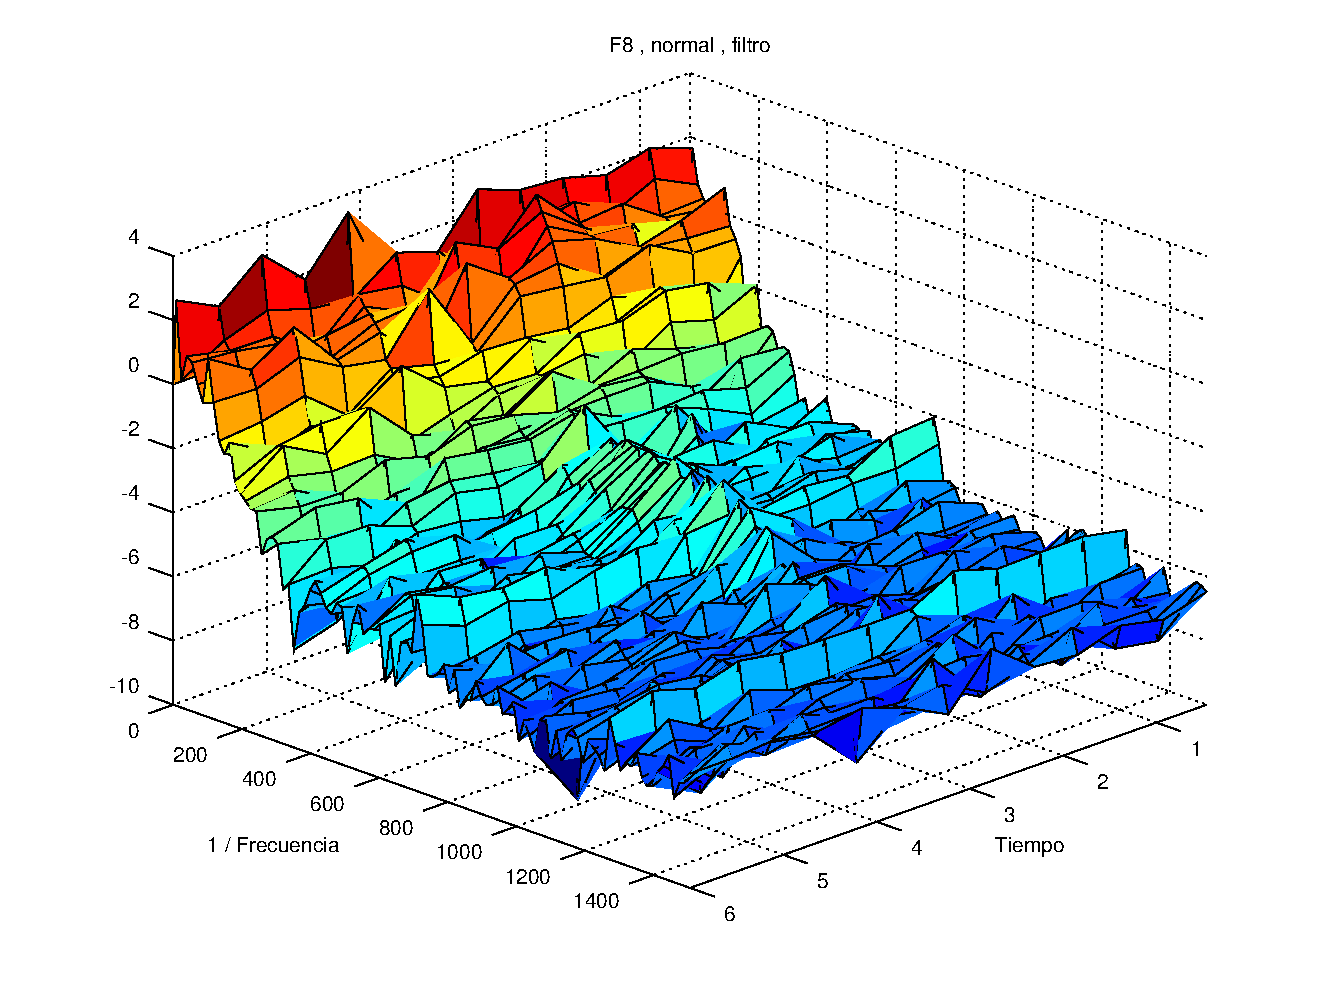
\includegraphics[width=0.5\linewidth]{n8f.pdf} 
&
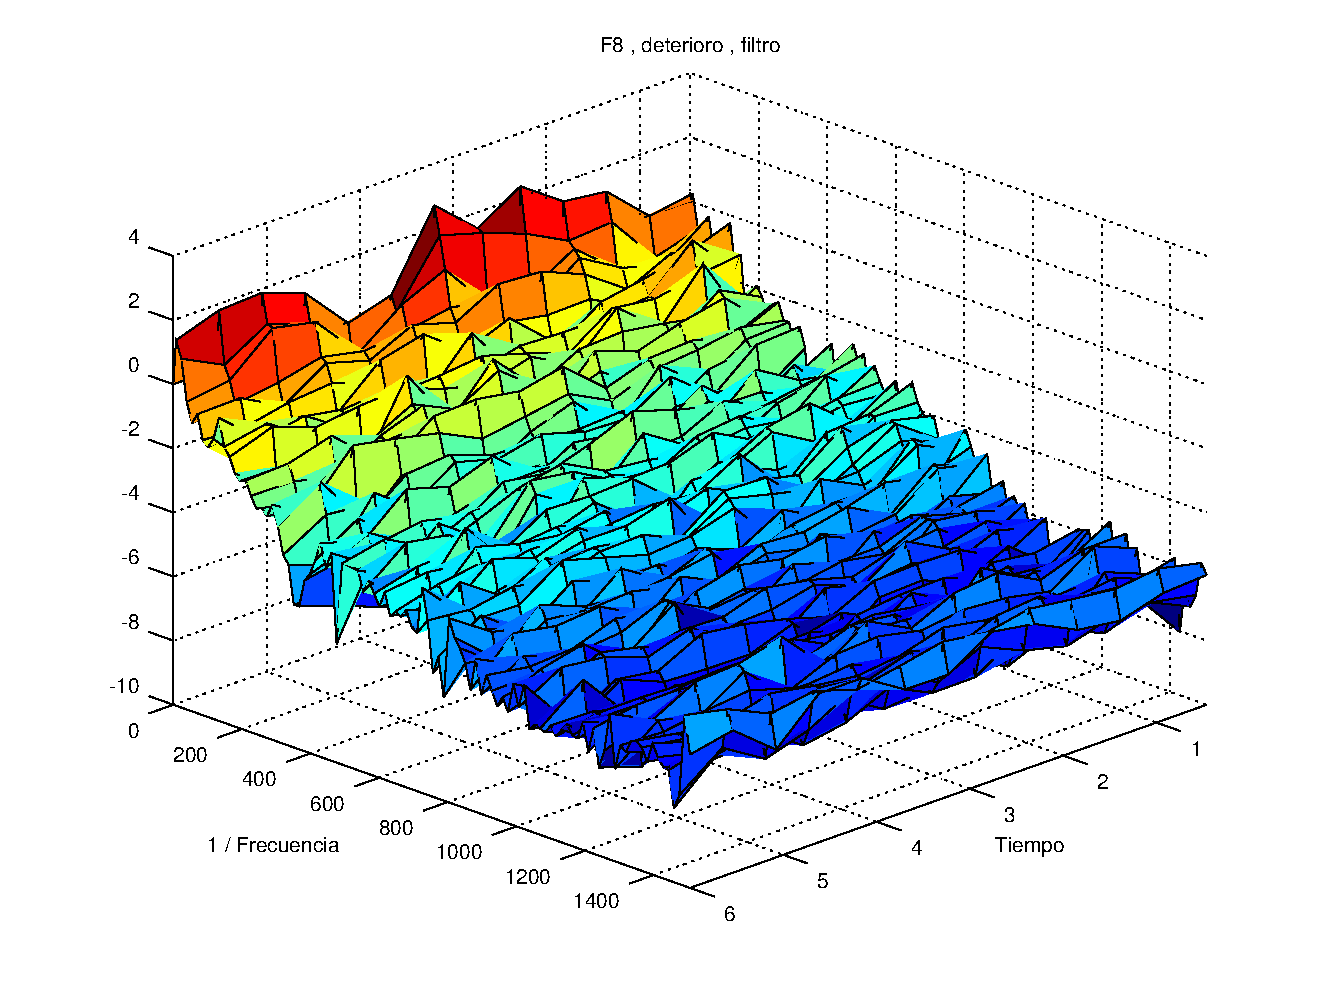
\includegraphics[width=0.5\linewidth]{d8f.pdf} 
\\
\begin{lstlisting}
T      : 0 
I+R    : 5.787895e-09 
T+I+R  : 0 
\end{lstlisting}
&
\begin{lstlisting}
T      : 0.00332259 
I+R    : 0.03502537 
T+I+R  : 0.01598073 
\end{lstlisting}
\end{tabular}

Este test se ha realizado para TODAS las epocas disponibles, pero como el test
es r\'apido s\'olo ha tardado 1 hora por sujeto usando una maquina potente [debo citar
los detalles tecnicos, y la cantidad de puntos procesados. Segun Nason (2012), el test PSR
tiene una velocidad del orden de $N log(N)$, con $N$ la cantidad de puntos procesados, y 
con lo cual es bastante mas rapido que otras pruebas].

%%%%%%%%%%%%%%%%%%%%%%%%%%%%%%%%%%%%%%%%%%%%%%%%%%%%%%%%%%%%%%%%%%%%%%%%%%%%%%%%%%%%%%%%%%%%%%%%%%%
%%%%%%%%%%%%%%%%%%%%%%%%%%%%%%%%%%%%%%%%%%%%%%%%%%%%%%%%%%%%%%%%%%%%%%%%%%%%%%%%%%%%%%%%%%%%%%%%%%%
%%%%%%%%%%%%%%%%%%%%%%%%%%%%%%%%%%%%%%%%%%%%%%%%%%%%%%%%%%%%%%%%%%%%%%%%%%%%%%%%%%%%%%%%%%%%%%%%%%%
%%%%%%%%%%%%%%%%%%%%%%%%%%%%%%%%%%%%%%%%%%%%%%%%%%%%%%%%%%%%%%%%%%%%%%%%%%%%%%%%%%%%%%%%%%%%%%%%%%%

\chapter{Resultados del test PSR}



\begin{figure}
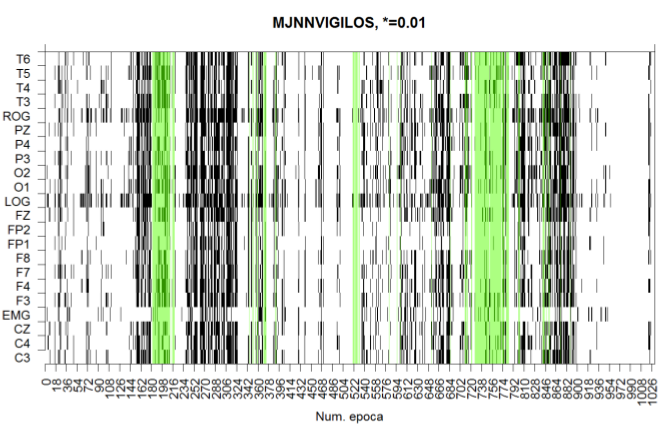
\includegraphics[width=\textwidth]{est01.png} 
\caption{Se muestran los resultados del test PSR de estacionariedad en el sujeto MJNN para las 1032 épocas de sueño en los
22 canales. En el eje horizontal se muestra el número de época, en el eje vertical se muestra al nombre del canal, de
modo que una fila tiene los resultados para un canal durante las diferentes épocas y una columna son los resultados
para todos los canales durante una época dada. En verde se han encerrado las épocas MOR.
Se consideró con un p-valor menor a 0.1 el rechazo de hipótesis nula: el registro en es no-estacionario (blanco),
mientras que el no-rechazo se consideró estacionario (negro).
Total de épocas: 1032 , Épocas MOR: 127}
\end{figure}

\begin{figure}
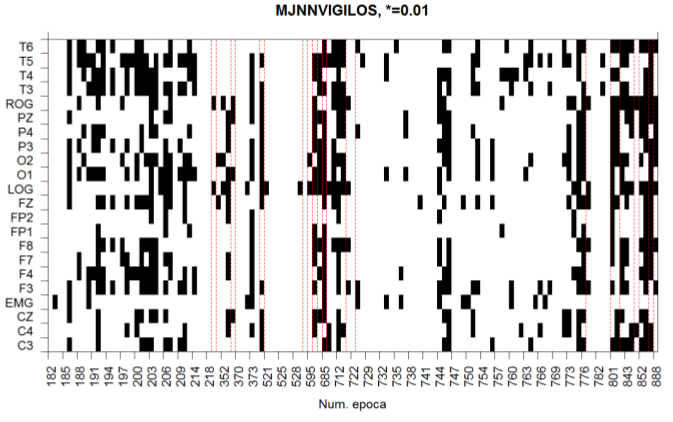
\includegraphics[width=\textwidth]{est02.png} 
\caption{En este gráfico sólo se ilustran épocas MOR. Las líneas punteadas separan bloques continuos.
Total de épocas: 1032 , Épocas MOR: 127}
\end{figure}

%%%%%%%%%%%%%%%%%%%%%%%%%%%%%%%%%%%%%%%%%%%%%%%%%%%%%%%%%%%%%%%%%%%%%%%%%%%%%%%%%%%%%%%%%%%%%%%%%%%
%%%%%%%%%%%%%%%%%%%%%%%%%%%%%%%%%%%%%%%%%%%%%%%%%%%%%%%%%%%%%%%%%%%%%%%%%%%%%%%%%%%%%%%%%%%%%%%%%%%